\documentclass[tikz,border=10pt]{standalone}
\usepackage{tikz}
\usetikzlibrary{positioning, shapes.geometric}

\begin{document}
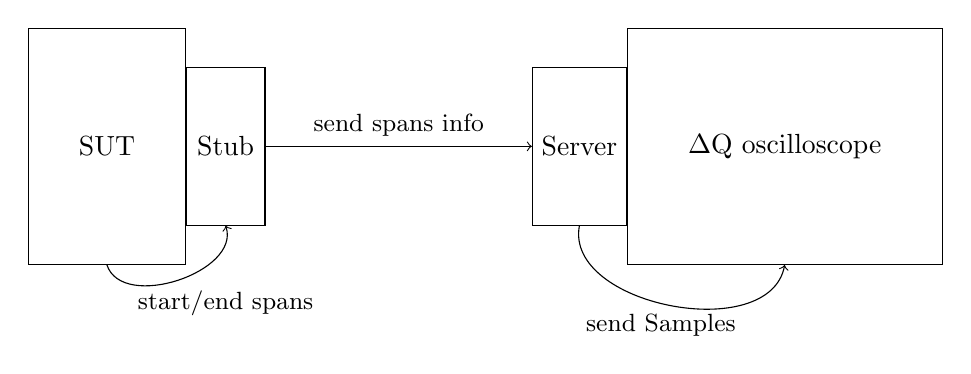
\begin{tikzpicture}

\node[rectangle,draw, minimum height = 3cm, minimum width = 2cm] (sut) at (-2, 0) {SUT};
\node[rectangle,draw, minimum height = 2cm, minimum width = 1cm, right of = sut, anchor = west] (stub) {Stub};

    \draw [->] (sut.south) to [bend right = 90] (stub.south) node[below=20pt] {\small start/end spans};

\node [rectangle, draw, minimum height = 2cm, minimum width = 1cm] (server) at (4, 0) {Server};
    \draw [->] (stub.east) -- (server.west) node[midway, above] {\small send spans info};
    \node [rectangle, draw, minimum height = 3cm, minimum width = 4cm, anchor = west] (osc) at(4.6, 0) {$\Delta$Q oscilloscope};
    \draw [->] (server.south) to [bend right = 90] (osc.south)  node[below left=20pt] {\small send Samples};
\end{tikzpicture}
\end{document}
